%!TEX root = ../lectures.tex

\topic{Intuition}

Differentiation, ultimately, is the problem of finding the slope\footnote{Or the rate of change, but since we are in only one variable these mean the same things.} of a function at some point.

\begin{figure}
	\centering
	\begin{subfigure}{0.4\textwidth}
		\centering
		\begin{tikzpicture}
			\begin{axis}[
				scale = 0.6,
				axis x line = middle,
				axis y line = middle,
				xmin = -1,
				xmax = 5,
				ymin = 0,
				ymax = 10,
				xlabel = $x$,
				ylabel = $y$,
				every axis x label/.style = {
					at = {(ticklabel* cs:1.01)},
					anchor = west,
				},
				every axis y label/.style = {
					at = {(ticklabel* cs:1.01)},
					anchor = south,
				},
				]
				\addplot[
				black,
				smooth,
				domain = -1:5,
				]{1.5*x+2};
				%\addplot[mark=*] coordinates {(3, 3)} node[pin=150:{$f(q)$}]{} ;
				%\addplot[mark=*] coordinates {(0.711, -0.945)} node[pin=-30:{$f(p)$}]{} ;
			\end{axis}
		\end{tikzpicture}
		\caption{Plot of a straight line.}
	\end{subfigure}
	\qquad
	\begin{subfigure}{0.4\textwidth}
		\centering
		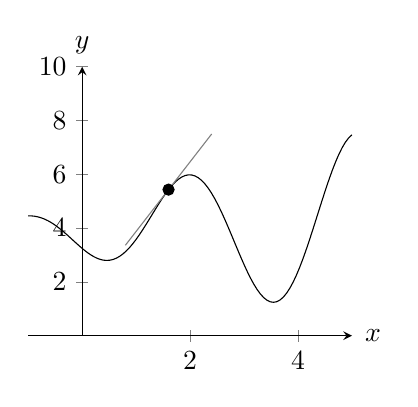
\begin{tikzpicture}
			\begin{axis}[
				scale = 0.6,
				axis x line = middle,
				axis y line = middle,
				xmin = -1,
				xmax = 5,
				ymin = 0,
				ymax = 10,
				xlabel = $x$,
				ylabel = $y$,
				every axis x label/.style = {
					at = {(ticklabel* cs:1.01)},
					anchor = west,
				},
				every axis y label/.style = {
					at = {(ticklabel* cs:1.01)},
					anchor = south,
				},
				]
				\addplot[
				black,
				samples = 100,
				domain = -1:5,
				]{0.5*(x+2)*sin((2*(x+2))r)+4};
				\addplot[
				gray,
				samples = 10,
				domain = 0.8:2.4
				]{2.5869*x + 1.28956};
				\addplot[mark=*] coordinates {(1.6, 5.4286)};
			\end{axis}
		\end{tikzpicture}
		\caption{Plot of a less straight line.}
		\label{lec3:notstraight}
	\end{subfigure}
	\caption{Examples of tangents of functions.}
\end{figure}

\noindent
If the function at hand is a (nonvertical) straight line, this is simple.
We read of a coefficient, or we compute rise over run, et cetera.

If, on the other hand, the function isn't a straight line, it can be slightly more complicated.
To do it, we simply fall back on what is essentially basic geometry in order to attempt to approximate the tangent line of the function at the point of interest.
We demonstrate by drawing on Figure \ref{lec3:notstraight} above, attempting to find the slope at $x = a$.

\begin{figure}
	\centering
	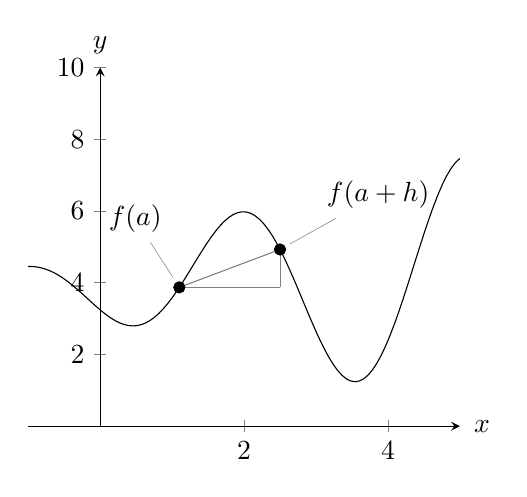
\begin{tikzpicture}
		\begin{axis}[
			scale = 0.8,
			axis x line = middle,
			axis y line = middle,
			xmin = -1,
			xmax = 5,
			ymin = 0,
			ymax = 10,
			xlabel = $x$,
			ylabel = $y$,
			every axis x label/.style = {
				at = {(ticklabel* cs:1.01)},
				anchor = west,
			},
			every axis y label/.style = {
				at = {(ticklabel* cs:1.01)},
				anchor = south,
			},
			]
			\addplot[
			black,
			samples = 100,
			domain = -1:5,
			]{0.5*(x+2)*sin((2*(x+2))r)+4};
			\addplot[
			gray,
			solid
			] coordinates {(1.1, 3.87121) (2.5, 4.92727)};
			\addplot[
			gray,
			solid
			] coordinates {(2.5, 4.92727) (2.5, 3.87121)};
			\addplot[
			gray,
			solid
			] coordinates {(2.5, 3.87121) (1.1, 3.87121)};
			\addplot[mark=*] coordinates {(1.1, 3.87121)} node[pin=100:{$f(a)$}]{} ;
			\addplot[mark=*] coordinates {(2.5, 4.92727)} node[pin=40:{$f(a + h)$}]{} ;
		\end{axis}
	\end{tikzpicture}
	\hfill
	\begin{tikzpicture}
		\draw[white] (1, 1.6);
		\draw (1.1, 3.87121) -- (3.5, 4.92727) -- node[right] {$f(a + h) - f(a)$} (3.5, 3.87121) -- node[below] {$a + h - a$} cycle;
		\draw (3.3, 3.87121) -- (3.3, 4.07121) -- (3.5, 4.07121);
	\end{tikzpicture}
	\caption{Constructing a difference quotient.}
\end{figure}

In other words, we let the point $(a, f(a))$ that we are interested in be one of the corners of a triangle, and pick some real number $h$ to construct another point $(a + h, f(a + h))$ on the curve.

As illustrated below, that creates a right triangle with base $a + h - a = h$ and height $f(a + h) - f(a)$. Hence to find the slope of the hypotenuse, we compute the rise over the run and arrive at
\[
	\text{slope} = \frac{\text{rise}}{\text{run}} = \frac{f(a + h) - f(a)}{h}
\]
of the line we just constructed.
The expression in the right-hand side is called a \keyword{difference quotient}\index{difference quotient}, or sometimes a \keyword{Newton quotient}\index{Newton quotient|see {difference quotient}}.

The trick is to now let $h$ go to $0$, but never quite reach it.
That way we will approach the slope at $x = a$, which is all right, because we know limits!

\topic{Definition and Computaitonal Rules}

Having done this we are ready to formalise the definition of the derivative.

\begin{definition}[Derivative, differentiability]
	The \keyword{derivative}\index{derivative} of a function $f$ is another function $f'$ defined by
	\[
		f'(x) = \lim_{h \to 0} \frac{f(x + h) - f(x)}{h}
	\]
	at all points $x$ for which the limit exists (in the sense that it is finite (and real, in this course)).

	If $f'(x)$ exists (at a given $x$), we say that $f$ is \keyword{differentiable}\index{differentiability} at $x$.
\end{definition}

\begin{remark}\label{lec3:singularpoint}
	The domain of $f'$ may be smaller than the domain of $f$, since $f$ need not be differentiable everywhere.
	Points where $f$ is not differentiable (and that aren't endpoints of closed intervals in the domain) are called \keyword{singular points}\index{singular point}.

	Moreover, note that the limit in the definition prevents a function from being differentiable at an isolated point.
	That is to say, for a function to be differentiable at a point, it must also be defined at some neighbourhood around that point.
\end{remark}

\begin{remark}
	An equivalent difference quotient limit that some people prefer is
	\[
		\lim_{x \to x_0} \frac{f(x) - f(x_0)}{x - x_0}.
	\]

	\noindent
	To see that this accomplishes the same thing, try drawing the corresponding picture.
\end{remark}

\begin{example}
	By definition, $f'(x)$ is the slope of $y = f(x)$ at the point $x = x_0$, where it exists.
	Therefore the tangent line to $y = f(x)$ at $(x_0, f(x_0))$ is
	\[
		y = f(x_0) + f'(x_0) (x - x_0). \qedhere
	\]
\end{example}

\noindent
It should be noted that the derivative comes with many different notations.
If our function is $y = f(x)$, the following all mean the same thing:
\[
	D_x y = y' = \frac{d y}{d x} = \frac{d}{d x} f = f' = D_x f = D f.
\]
In some of these, the variable $x$ is implied, whereas in others it is explicit.
For us, doing calculus in only one variable, there will probably never be any ambiguity in not specifying the variable, but once one starts doing calculus in more variables, it becomes a very good idea to specify.

Finally, before we go on to prove various interesting properties of the derivative, we make a note about what happens at endpoints of closed intervals in the domains of functions, thereby also clarifying what we meant by the parentheses in Remark \ref{lec3:singularpoint} above.

\begin{remark}[Left and right derivatives]
	Suppose our function $f$ that we wish to differentiate is defined on a closed interval $[a, b]$.
	We have a problem if we try to compute $f'(a)$ or $f'(b)$.

	Consider, for instance, $x = a$.
	What happens if $h < 0$ in the difference quotient?
	Well, in $f(a + h)$ we have $x = a + h < a$, and for such a value of $x$ the function $f$ isn't defined.

	The solution is to use one-sided limits where appropriate, to define \keyword{left} and \keyword{right derivatives}\index{derivative!left}\index{derivative!right}:
	\[
		f'_+(a) = \lim_{h \to 0^+} \frac{f(a + h) - f(a)}{h} \qquad \text{and} \qquad f'_- (b) = \lim_{h \to 0^-} \frac{f(b + h) - f(b)}{h}.
	\]
\end{remark}

\noindent
There is an important connection between differentiability and continuity.

\begin{theorem}\label{lec3:diffimpliescont}
	If $f$ is differentiable at $x$, then it is also continuous at $x$.
\end{theorem}

\begin{proof}
	Since $f$ is differentiable at $x$, the limit
	\[
		f'(x) = \lim_{h \to 0} \frac{f(x + h) - f(x)}{h}
	\]
	exists. We then take the difference between $\lim\limits_{h \to 0} f(x + h)$ and $f(x)$:
	\begin{align*}
		\lim\limits_{h \to 0} (f(x + h)) - f(x) & = \lim_{h \to 0} (f(x + h) - f(x)) = \lim_{h \to 0} \frac{f(x + h) - f(x)}{h} \cdot h  \\
		                                        & = \lim_{h \to 0} \frac{f(x + h) - f(x)}{h} \cdot \lim_{h \to 0} h = f'(x) \cdot 0 = 0.
	\end{align*}
	This means that the distance between the limit of $f$ at $x$ and $f(x)$ is 0, whereby they are equal, so by definition $f$ is continuous at $x$.
\end{proof}

\noindent
The converse is not true, i.e. there exists continuous functions that aren't differentiable.

\begin{counterexample}
	Consider the absolute value function $f(x) = \abs{x}$.
	This function is continuous at the point $x = 0$ ($\delta = \varepsilon$ works fine in the definition of continuity, for instance), but it is not differentiable there, since the the limit defining the derivative doesn't exist there; from the left the limit is $-1$, whereas from the right the limit is $1$.
\end{counterexample}

\noindent
We now formulate and prove various computational rules of derivatives that we will continue using throughout the course.

\begin{theorem}[Addition, subtraction, and multiplication by constant]
	Let $f$ and $g$ be differentiable functions at $x$, and let $k$ be some constant.
	Then $f + g$, $f - g$, and $k f$ are all differentiable at $x$, and
	\begin{romanlist}
		\item $(f + g)'(x) = f'(x) + g'(x)$;
		\item $(f - g)'(x) = f'(x) - g'(x)$; and
		\item $(k f)'(x) = k f'(x)$.
	\end{romanlist}
\end{theorem}

\begin{proof}
	We simply rearrange the difference quotients and use our rules for limits.
	For \fakeitemref{1} and \fakeitemref{2}, this becomes
	\begin{align*}
		(f \pm g)'(x) & = \lim_{h \to 0} \frac{(f \pm g)(x + h) - (f \pm g)(x)}{h}                                                   \\
		              & = \lim_{h \to 0} \frac{f(x + h) \pm g(x + h) - (f(x) \pm g(x))}{h}                                           \\
		              & = \lim_{h \to 0} \frac{f(x + h) - f(x)}{h} \pm \lim_{h \to 0} \frac{(g(x + h) - g(x))}{h} = f'(x) \pm g'(x).
	\end{align*}

	\noindent
	For \fakeitemref{3}, we get a similarly trivial computation:
	\[
		(k f)'(x) = \lim_{h \to 0} \frac{k f(x + h) - k f(x)}{h} = k \cdot \lim_{h \to 0} \frac{f(x + h) - f(x)}{h} = k f'(x). \qedhere
	\]
\end{proof}

\noindent
What happens when multiplying two functions together is perhaps less intuitive:

\begin{theorem}[Product rule]
	Let $f$ and $g$ be functions differentiable at $x$.
	Then $f g$ is also differentiable at $x$, and
	\[
		(f g)'(x) = f'(x) g(x) + f(x) g'(x).
	\]
\end{theorem}

\begin{proof}
	We study the difference quotient and add $0$ in a clever way:
	\begin{align*}
		(f g)'(x) & = \lim_{h \to 0} \frac{f(x + h) g(x + h) - f(x) g(x)}{h}                                                         \\
		          & = \lim_{h \to 0} \frac{f(x + h) g(x + h) - f(x) g(x + h) + f(x) g(x + h) - f(x) g(x)}{h}                         \\
		          & = \lim_{h \to 0} \Big ( \frac{f(x + h) - f(x)}{h} \cdot g(x + h) + f(x) \cdot \frac{g(x + h) - g(x)}{h} \Big )   \\
		          & = \lim_{h \to 0} \frac{f(x + h) - f(x)}{h} \cdot g(x + h) + \lim_{h \to 0} f(x) \cdot \frac{g(x + h) - g(x)}{h}  \\
		          & = \lim_{h \to 0} \frac{f(x + h) - f(x)}{h} \cdot g(x + h) + f(x) \cdot \lim_{h \to 0} \frac{g(x + h) - g(x)}{h}.
	\end{align*}
	The crucial last step is to now recall Theorem \ref{lec3:diffimpliescont}, whereby $g$ is continuous, and therefore the above becomes
	\[
		(f g)'(x) = f'(x) g(x) + f(x) g'(x). \qedhere
	\]
\end{proof}

\noindent
Dealing with quotients is maybe even less intuitive.

\begin{theorem}[Quotient rule]
	If $f$ and $g$ are differentiable functions at $x$ and $g(x) \neq 0$, then the quotient $f / g$ is differentiable at $x$, and
	\[
		\Big ( \frac{f}{g} \Big )'(x) = \frac{f'(x) g(x) - f(x) g'(x)}{(g(x))^2}.
	\]
\end{theorem}

\noindent
To prove it, we first prove an easier result.

\begin{lemma}[Reciprocal rule]
	If $g$ is differentiable at $x$ with $g(x) \neq 0$, then $1 / g$ is differentiable at $x$ and
	\[
		\Big ( \frac{1}{g} \Big )' = -\frac{g'(x)}{(g(x))^2}.
	\]
\end{lemma}

\begin{proof}
	The trick lies entirely in writing the numerator with common denominator:
	\begin{align*}
		\frac{d}{d x} \Big ( \frac{1}{g(x)} \Big ) & = \lim_{h \to 0} \frac{\frac{1}{g(x + h)} - \frac{1}{g(x)}}{h} = \lim_{h \to 0} \frac{\frac{g(x) - g(x + h)}{g(x + h) g(x)}}{h} \\
		                                           & = \lim_{h \to 0} \frac{g(x) - g(x + h)}{h g(x + h) g(x)} = - \lim_{h \to 0} \frac{g(x + h) - g(x)}{h g(x + h) g(x)}             \\
		                                           & = - \lim_{h \to 0} \frac{1}{g(x) g(x + h)} \cdot \frac{g(x + h) - g(x)}{h}                                                      \\
		                                           & = - \frac{g'(x)}{(g(x))^2}. \qedhere
	\end{align*}
\end{proof}

\noindent
With this at our disposal proving the quotient rule becomes a special case of the product rule.

\begin{proof}[Proof of the Quotient rule]
	We write $f / g$ as $f \cdot 1 / g$ and use the product rule:
	\begin{align*}
		\frac{d}{d x} \Big ( \frac{f(x)}{g(x)} \Big ) & = \frac{d}{d x} \Big ( f(x) \cdot \frac{1}{g(x)} \Big ) = f'(x) \frac{1}{g(x)} + f(x) \Big ( \frac{- g'(x)}{(g(x))^2} \Big ) \\
		                                              & = \frac{f'(x) g(x) - f(x) g'(x)}{(g(x))^2}. \qedhere
	\end{align*}
\end{proof}

\noindent
In keeping with how we dealt with continuity, after addition, subtraction, multiplication and division comes composition.

\begin{theorem}[Chain rule]
	If $f$ is differentiable at $y = g(x)$, and $g$ is differentiable at $x$, then $f \circ g$ is differentiable at $x$ and $(f \circ g)'(x) = f'(g(x)) g'(x)$.
\end{theorem}

\begin{proof}
	We construct a slightly tricky function $E$, defined as
	\[
		E(k) = \begin{cases}
		0, & \text{if}~ k = 0 \\
		\frac{f(y + k) - f(y)}{k} - f'(y), & \text{if}~ k \neq 0.
		\end{cases}
	\]
	Notice how
	\[
		\lim_{k \to 0} E(k) = \lim_{k \to 0} \frac{f(y + k) - f(y)}{k} - \lim_{k \to 0} f'(y) = f'(y) - f'(y) = 0 = E(0),
	\]
	meaning that $E(k)$ is continuous at $k = 0$.
	Moreover
	\[
		E(k) + f'(y) = \frac{f(y + k) - f(y)}{k},
	\]
	which implies that
	\[
		f(y + k) - f(y) = (E(k) + f'(y)) \cdot k.
	\]

	\noindent
	If we now take $y = g(x)$ and $k = g(x + h) - g(x)$, meaning that $y + k = g(x + h)$, and inserting this into the above equation we get
	\begin{equation}\label{lec3:chaindiff}
		f(g(x + h)) - f(g(x)) = \big (f'(g(x)) + E(k) \big ) (g(x + h) - g(x)).
	\end{equation}

	\noindent
	By assumption $g$ is differentiable at $x$, meaning that
	\[
		g'(x) = \lim_{h \to 0} \frac{g(x + h) - g(x)}{h},
	\]
	and also that $g$ is continuous at $x$, whereby $\lim\limits_{h \to 0} g(x + h) - g(x) = 0$.

	We are now ready to compute the limit of the difference quotient of the composition, using Equation \ref{lec3:chaindiff} straight away:
	\[
		\frac{d}{d x} f(g(x)) = \lim_{h \to 0} \frac{f(g(x + h)) - f(g(x))}{h} = \lim_{h \to 0} (f'(g(x)) + E(k)) \, \frac{g(x + h) - g(x)}{h}.
	\]
	Now since $E$ is continuous at $0 = \lim\limits_{h \to 0} g(x + h) - g(x) = \lim\limits_{h \to 0} k$, we have
	\[
		\lim_{h \to 0} E(k) = E \Big ( \lim_{h \to 0} k \Big ) = E(0) = 0,
	\]
	whereby the above becomes
	\[
		\frac{d}{d x} f(g(x)) = f'(g(x)) g'(x). \qedhere
	\]
\end{proof}

\topic{Derivatives of Trigonometric Functions}

We state without proof that $\sin$ and $\cos$ are continuous functions everywhere.

Moreover, we claim that $\lim\limits_{x \to 0} \sin(x) = 0$ and $\lim\limits_{x \to 0} \cos(x) = 1$.

\begin{exercise}
	Try to prove it.

	\emph{Hint: for the first one, use $\sin(\alpha + \beta) - \sin(\alpha - \beta) = 2 \cos(\alpha)\sin(\beta)$ to manipulate $\abs{\sin(x) - \sin(a)}$ into a single $\sin$.
	For both this and the $\sin$ limit, it will help to prove that $0 \leq \abs{\sin(x)} \leq \abs{x}$.}
\end{exercise}

\noindent
In closing, we will prove an important limit, which we will use next time to compute the derivatives of $\sin$ and $\cos$.

\begin{lemma}
	$\displaystyle \lim_{x \to 0} \frac{\sin(x)}{x} = 1$.
\end{lemma}

\begin{proof}
	This proof relies very much on the geometrical construction of $\sin$ and $\tan$ found in Figure \ref{lec3:sinx/x}.
	Let $0 < x < \pi / 2$.

	\begin{figure}[t]
		\centering
		\begin{tikzpicture}[scale = 1]

			\draw[gray,-latex](-0.4, 0) -- (5, 0); % x-axis
			\draw[gray,-latex](0, -0.4) -- (0, 5); % y-axis
			\pic{circle arc = 0:90:4}; % Unit circle

			\draw (0, 0) node[below, fill = white]{$A$} coordinate (A);
			\filldraw (A) circle[radius = 1.5pt];

			\draw (4, 0) node[below right]{$B$} coordinate (B);
			\filldraw (B) circle[radius = 1.5pt];

			\draw (50:4) node[above]{$C$} coordinate (C);
			\filldraw (C) circle[radius = 1.5pt];

			\draw (4, 4.767) node[right]{$D$} coordinate (D);
			\filldraw (D) circle[radius = 1.5pt];

			\draw[black] (A) -- (D) -- (B) -- (C);
			\draw[<->] (0.2, -0.25) -- node[midway, fill = white]{$1$} (3.9, -0.25);
			\draw[<->] (4.25, 0.1) -- node[midway, right, fill = white]{$\tan(x)$} (4.25, 4.417);
			\draw[<->] (2.571, 0.2) -- node[midway, fill = white]{$\sin(x)$} (2.571, 2.814);

			\pic[draw, angle eccentricity=1.2, angle radius = 0.7cm, "$\quad\!x$"]{angle=B--A--D};
		\end{tikzpicture}
		\caption{A geometrical representation of $\sin$ and $\tan$ on the unit circle.}
		\label{lec3:sinx/x}
	\end{figure}

	We make three claims:
	\begin{romanlist}
		\item The area of the triangle $\triangle A B C$ is $\frac{1}{2} \sin(x)$ (since $\sin(x)$ is its height).
		\item The area of the sector $A B C$ is $\frac{1}{2} x$.
		\item The area of the triangle $\triangle A B D$ is $\frac{1}{2} \tan(x)$.
	\end{romanlist}

	\noindent
	Moreover, it is clear that these areas are in ascending order as listed, i.e.
	\[
		\frac{1}{2} \sin(x) \leq \frac{1}{2} x \leq \frac{1}{2} \tan(x).
	\]
	If we divide by $\frac{1}{2} \sin(x)$, which is positive since $0 < x < \pi / 2$, we then get
	\[
		1 \leq \frac{x}{\sin(x)} \leq \frac{1}{\cos(x)}.
	\]
	Finally we take reciprocals, thereby reversing the inequalities,
	\[
		\cos(x) \leq \frac{\sin(x)}{x} \leq 1.
	\]

	\noindent
	Note how $1$, $\sin(x) / x$, and $\cos(x)$ are all even functions, so this chain of inequalities is true also for $-\pi / 2 < x < 0$ by symmetry.
	This is good, because it allows us to consider the two-sided limit we are interested in, despite the geometric picture only discussing positive $x$.

	Finally we remark that since $\lim\limits_{x \to 0} \cos(x) = 1$, the Squeeze theorem tells us that
	\[
		\lim_{x \to 0} \frac{\sin(x)}{x} = 1,
	\]
	as desired.
\end{proof}
